% \section{Outline}

In his video essay, A Future of Medicine, Dr. Bernard postulates on a world that views our current system of evidence based medicine, as we see European plague doctors. In short, his thesis thereto is that simulations will replace modern day drug trials. 

Furthermore, in his talk, he points out two outstanding issues with our current system of evidence based medicine.

\begin{enumerate}
    \item The first stems from human trials, where issues may arise if there is a disparity in efficacy, where one group may be effectively condemned to death.\textsuperscript{(Harmon)}
    \item The second pertains to issues in generalizing data from human trials for predicting outcome for a given individual. For instance, as Dr. Bernard points out, if a trial was done on a bunch of men, clinical experience suggests that there will be differences for women taking the same medication.\textsuperscript{(Bernard)} Nowadays, trials are required to include notable age, gender, and race/ethnicity demographics. But as Kravitz pointed out, ``[this] may do nothing but ensure that the estimates for any one subgroup are unreliable due to small numbers''. In the very same paper, Kravitz coined this phenomena, the ``Heterogeneity of Treatment Effects''. 
\end{enumerate}

If you're still unconvinced. Even if you happen to be well represented in this respect, some have argued that ``all of us fall into this category for some traits''\textsuperscript{(Beckmann)}. 

From here, with the problem outlined. Let's consider an alternative. What if, instead of running a trial on thousands of disperse persons. What if you were simply cloned, hundreds of thousands of times, and therein, we performed hundreds of thousands of trials, forming a stochastic model that likewise predicts outcome for some given treatment? To this, you may ask, how exactly do we run hundreds of thousands of trials of my identical clones?

We run computer simulations, as Dr. Bernard proposed. Although what Dr. Bernard proposed, was essentially a thought experiment, explicitly regarding this as something that probably won't be viable in our lifetime. Conversely, my research paper will say otherwise. In a thesis that forgoes a multitude of modern innovations, from the von-neumann architecture, digital computer architectures, numerical precision, and ultimately, generality. In favor of analog computer architectures that more directly models the natural phenomena it's tasked with simulating.  Notably, analog computing more efficiency solves the differential equations governing the various processes taking place within your body, in a manner that conventional computer architectures are fundamentally ill adept at. Which, in this respect, Sarpeshkar argues that analog computing is more efficient in terms of energy, time (computation) and space (memory and program installation).

To explain why, imagine we somehow needed to compute one instruction for each atom, for each cell, in the human body. Which would then amount to $4 \mathrm{x} 10^{27}$ instructions. To imagine this in terms of time. Consider first, simply the latency overhead incurred when your processing hardware and main memory is physically separated from each other, and therefore, each instruction must first read some datum from main memory. Lets say this overhead is $100\mathrm{ns}$ per instruction. Then latency overhead alone will amount to $4\;\mathrm{x}\;10^{20}$ seconds, or in other words, latency overhead alone will total $12,683,916,800,000$ years per evolution. Therefore, the current von neumann paradigm won't suffice. But alas, this is a ludicrous exercise for a multitude of reasons. Because, for instance, what is meant by one instruction per atom? For each evolution, can the state of each atom be computed without considering neighboring interactions?

But crucially, consider, for instance, the following digram that implements $\ddot{y} = -y$. 

\begin{figure}[H]
    \centering
    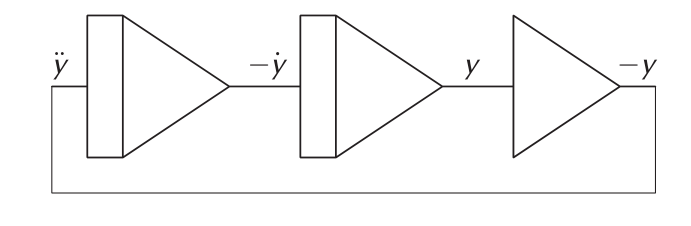
\includegraphics[width=0.6\linewidth]{../assets/analogue-computing-fun-differential-equations.png}
    \caption{Source: \url{https://chalkdustmagazine.com/features/analogue-computing-fun-differential-equations/}. (Note that this is missing initial conditions.)}
    \label{Image Label}
\end{figure}

This program works without even requiring stored computer memory.

In the above figure, the leftmost elements are the integrators, while the rightmost element is called the summer, and each elements implicitly flips the sign. Personally, there is an elegant economy to the above diagram, and furthermore, it implements such without requiring stored computer memory, and this itself is notable (as I will try to explain shortly). In contrast, implementing the same processes on digital computer architectures would require significantly more infrastructure in implementing the same mathematical laws in terms of manipulations of arbitrary symbols. Which obviously increases overall costs, size, energy requirements, and so forth.

The reason for our fixation on differential equations is because this is the mathematical framework in which we typically model systems in nature. But not just the sciences, such is also pervasive throughout engineering, including electrical circuits. Therefore, as I like to imagine, it's not too much of a stretch to go from modeling to simulation.

In contrast, as MacLennan argued, in digital computation, quantities are rather arbitrary symbols that have no direct relationship to the physical systems that such may be tasked with simulating. In contrast, generally speaking, analog and physical phenomena are governed and defined by the same mathematical laws. Or as MacLennan put it, ``the computational quantities are proportional to the modeled quantities.''\textsuperscript{(MacLennan)}

This is due, not to processing performance, but as Sarpeshkar argues, in information theory. That is, digital computation in contrast, while built upon analog mediums, forgoes most of the real estate therein for a limited set of gates defined in terms of a mere bit, in a single multi-bit analog channel. Conversely, in allowing full utilization of the unclaimed and unexploited real estate therefrom, in further expanding our conception of computation to more than mere logic, new applications may potentially become commercially viable. Such as perhaps, simulating the molecular interactions within cells, to tissues, to entire organ systems, to perhaps, entire persons.

I first heard about such speculations from a TED-X talk by a man called Rahul Sarpeshkar (Professor of Engineering, Thomas E. Kurtz Professor, Professor of Microbiology \& Immunology, Professor of Physics, Professor of Molecular \& Systems Biology). In his talk, Sarpeshkar discussed the prospects of analog computing for solving differential equations in a manner that far outpaces the capabilities of digital computers, and furthermore, he claimed that we could viably simulate an entire person if we built an analog computer that spanned the size of the given auditorium.

The negative side of analog computing lies in precision, which is typically bounded to just three or four bits of precision.

But, In this respect, Sarpeshkar and Teo have argued that the power efficiency of cells, stems from forgoing precision to the maxim possible extent that the operations therein affords. Which as Teo argues, pushes cells ``near the thermodynamic limits of physics''. 

Furthermore, some authors have argued that there is, as I have put it, an isomorphism between chemistry and electric analog circuitry, that to me, makes me think that this thesis is ideal for the given problem. For instance, as Teo wrote
\begin{quotation}
    ``There is a deep connection between ‘electronics’, which is about the controlled, relatively long-range motions of electrons be- tween devices, and ‘chemistry’, which is about the controlled, relatively short-range motions of electrons between atoms and molecules.''\textsuperscript{(Teo)}
\end{quotation}

That is, we have a model that can manifest in chemical systems and electric analog circuitry, from this link between electronics (simulation) and chemistry (e.g. biochemical computation). Alternatively, as Sarpeshkar wrote,
\begin{quotation}
    ``There are striking similarities between chemical-reaction dynamics (figure 3a) and electronic current flow in the subthreshold regime of transistor operation (figure 3b): electron concentration at the source is analogous to reactant concentration; electron concentration at the drain is analogous to product concentration; forward and reverse current flows in the transistor are analogous to forward and reverse reaction rates in a chemical reaction; the forward and reverse currents in a transistor are exponential in voltage differences at its terminals analogous to reaction rates being exponential in the free-energy differences in a chemical reaction; increases in gate voltage lower energy barriers in a transistor increasing current flow analogous to the effects of enzymes or catalysts in chemical reactions that increase reaction rates; and the stochastics of the Poisson shot noise in subthreshold transistors are analogous to the stochastics of molecular shot noise in reactions. [...] The logarithmic dependence of the electrochemical potential in chemical concentration or of current enables one to map log-domain analog transistor circuit motifs in electronics to log-domain analog molecular circuit motifs in cells and vice versa.''\textsuperscript{(Sarpeshkar)}
\end{quotation}

More generally, what has traditionally encumbered analog computing is noise interference. But in a similar manner, Sarpeshkar likewise argues that the noise interference that has traditionally encumbered analog computing is, in fact, a benefit. This is because when running stochastic processes, we essentially get randomness for free. This is in contrast to simulating randomness in digital computers, which imposes significant comparative overhead.

Obviously, there also exists significant costs to developing and manufacturing unproven technology. But, remember when we spoke of a tradeoff between resource expenditure and accuracy? When we speak of costs, we have to consider what we are proposing in contrast to the current norm, and in this regard, if you desire accuracy, currently it's said that you're limited to simulating the effects of small molecules, on supercomputers or other high performance computing (HPC) environments where the installation and operational costs therein are significant.

Considering for instance, Tianhe-1A: initial costs amounted to $\$88$ million dollars, and another $\$20$ million dollars is spent, per year, on power consumption.\textsuperscript{(Tianhe-1)} 

Which means after four years, power consumption alone become the most significant cost factor. In contrast, Trafton argues that, ``[in] one second, a [typical] cell performs about 10 million energy-consuming chemical reactions, which altogether require about one picowatt (one millionth millionth of a watt) of power.''\textsuperscript{(Trafton)}

Even for one of the more power hungry human organs (relative to weight), the human brain, requires a mere 12 to 15 watts of power, to sustain trillions of operations therein. (Which is about the power consumption of a lightbulb.) The energy efficiency therefrom, as Sarpeshkar proposes, is again, the product of forgoing high precision operations in favor of low precision analog computation with feedback mechanisms.



In this manner, even an approximation of the best case scenario leads to a platform that favors experimentation and iteration, by both small and underfunded terms, to billion dollar pharmaceutical companies. Which I argue, has far reaching implications. Because this reduces modeling to programming, and from programming, abstraction. Why does this matter?

For a multitude of reasons. First, humans are utterly unrivaled when it comes to natures ability to self assemble into sophisticated structures (including ourselves).

That is, we can plant a seed, and grow a tree, but planting a seed to grow a house is unfathomable. Just as unfathomable as designing robots to kill cancer cells, which again, nature has parallels. 

Presumably this is due to complex factors that may be abstracted within my proposed computer architecture. (Remember that aforementioned isomorphism?) When we abstract, we may sometimes reduce `complex' things into simpler, more conceptually `discrete' things. Which therein, due to this simpler nature, may further permit others to effectively build upon such, and therein, may create something more sophisticated, perhaps even, greater than the sum of it's components. 

That is, a system where discrete units build upon other discrete units and therein produce more complex non-discrete units. This system permits for abstraction, so complex non-discrete units may be abstracted into simple discrete units. Thereafter this process of production and abstraction enables further production and abstraction and so forth. Each iteration or generation may be considered to be more sophisticated than prior generations, given that each generation is a product of prior generations… From this analogy, you can imagine these bottom-up and cumulative processes will eventually give rise to very sophisticated products, and perhaps one day, akin to how emergence gives rise to the complexity found in nature.

From personal experience, my \url{https://imager.io} project wouldn’t be possible without the various open source components it’s built upon. Simply because my time is finite, and especially because lower-level encoding details are just \textbf{too complicated for me to understand and implement on my own}. I am nevertheless able to compose such components into a larger and more sophisticated end product, from the preexisting output of resources and information from the global open source, software community. Overall added value that may be considered to be greater than the sum of its components, and therefore emergent in a manner of speaking. In an old English paper I likened the open source community as ``the printing press of computable knowledge'', and perhaps even more significant than the advent of the printing press itself, because as the industrial revolution introduced a force multiplier of human muscle, so too does abstraction introduce a force multiplier of the human mind.

Because, while a book may describe a life’s work in mathematics and applications therein, the medium is itself rather passive. A book may describe a life’s work in applied mathematics, yet a mind is required to manifest its application. Whereas, imagine a medium where the most knowledgeable of experts can record their understanding of a given domain as functions that map problems to solutions, in a manner that can be utilized by any layperson, and thereafter this record can be reapplied, reused, and so forth, forever thereafter, and, in this manner, what are the ramifications of such?

Furthermore, if you can build upon abstracted systems written by experts, where these abstractions mask complexity, we may then presume that the overall barrier to entry will drop. That is again, if laypersons are able to built upon abstracted systems in a manner that doesn't require an expert understanding or formal education in such (and presumably in a manner akin to my aforementioned \url{https://imager.io} story). But on the other end, if the barrier to entry is lower, this implies reduced costs, and therefore, we may likewise see significant cost savings in industries built upon such, perhaps in a manner akin to using ``higher level'' programming languages for applicable problems. 




















